\chapter{Overview}
\sdr is a software-defined radio based on Microsemi's SmartFusion. Unlike common FPGAs, the SmartFusion
is a device which incorporates a hard core ARM Cortex M3 and a flash-based FPGA. Flash-based FPGA
technology offers low static power, no reconfiguration in boot stage and memory retention when in
power down mode. These benefits make it a better candidate for low-power wireless research. We present
the \sdr, a true battery-powered SDR platform which is suitable for portable and deployable hand held
device research.
\section{Features}
\begin{enumerate}
	\item 2.4 - 2.5~GHz ISM band
	\item Dual channel 80~MS/s, 8-bits ADC
	\item Dual channel 40~MS/s, 8-bits DAC
	\item 16~MB External PSRAM
	\item 8~MB External Flash
	\item $\pm$3~ppm TXCO
	\item Ethernet, USB interfaces
	\item 24 User defined IO, 8 LEDs and 4 switches
	\item Battery-powered
\end{enumerate}

\begin{figure}[h]
\centering
	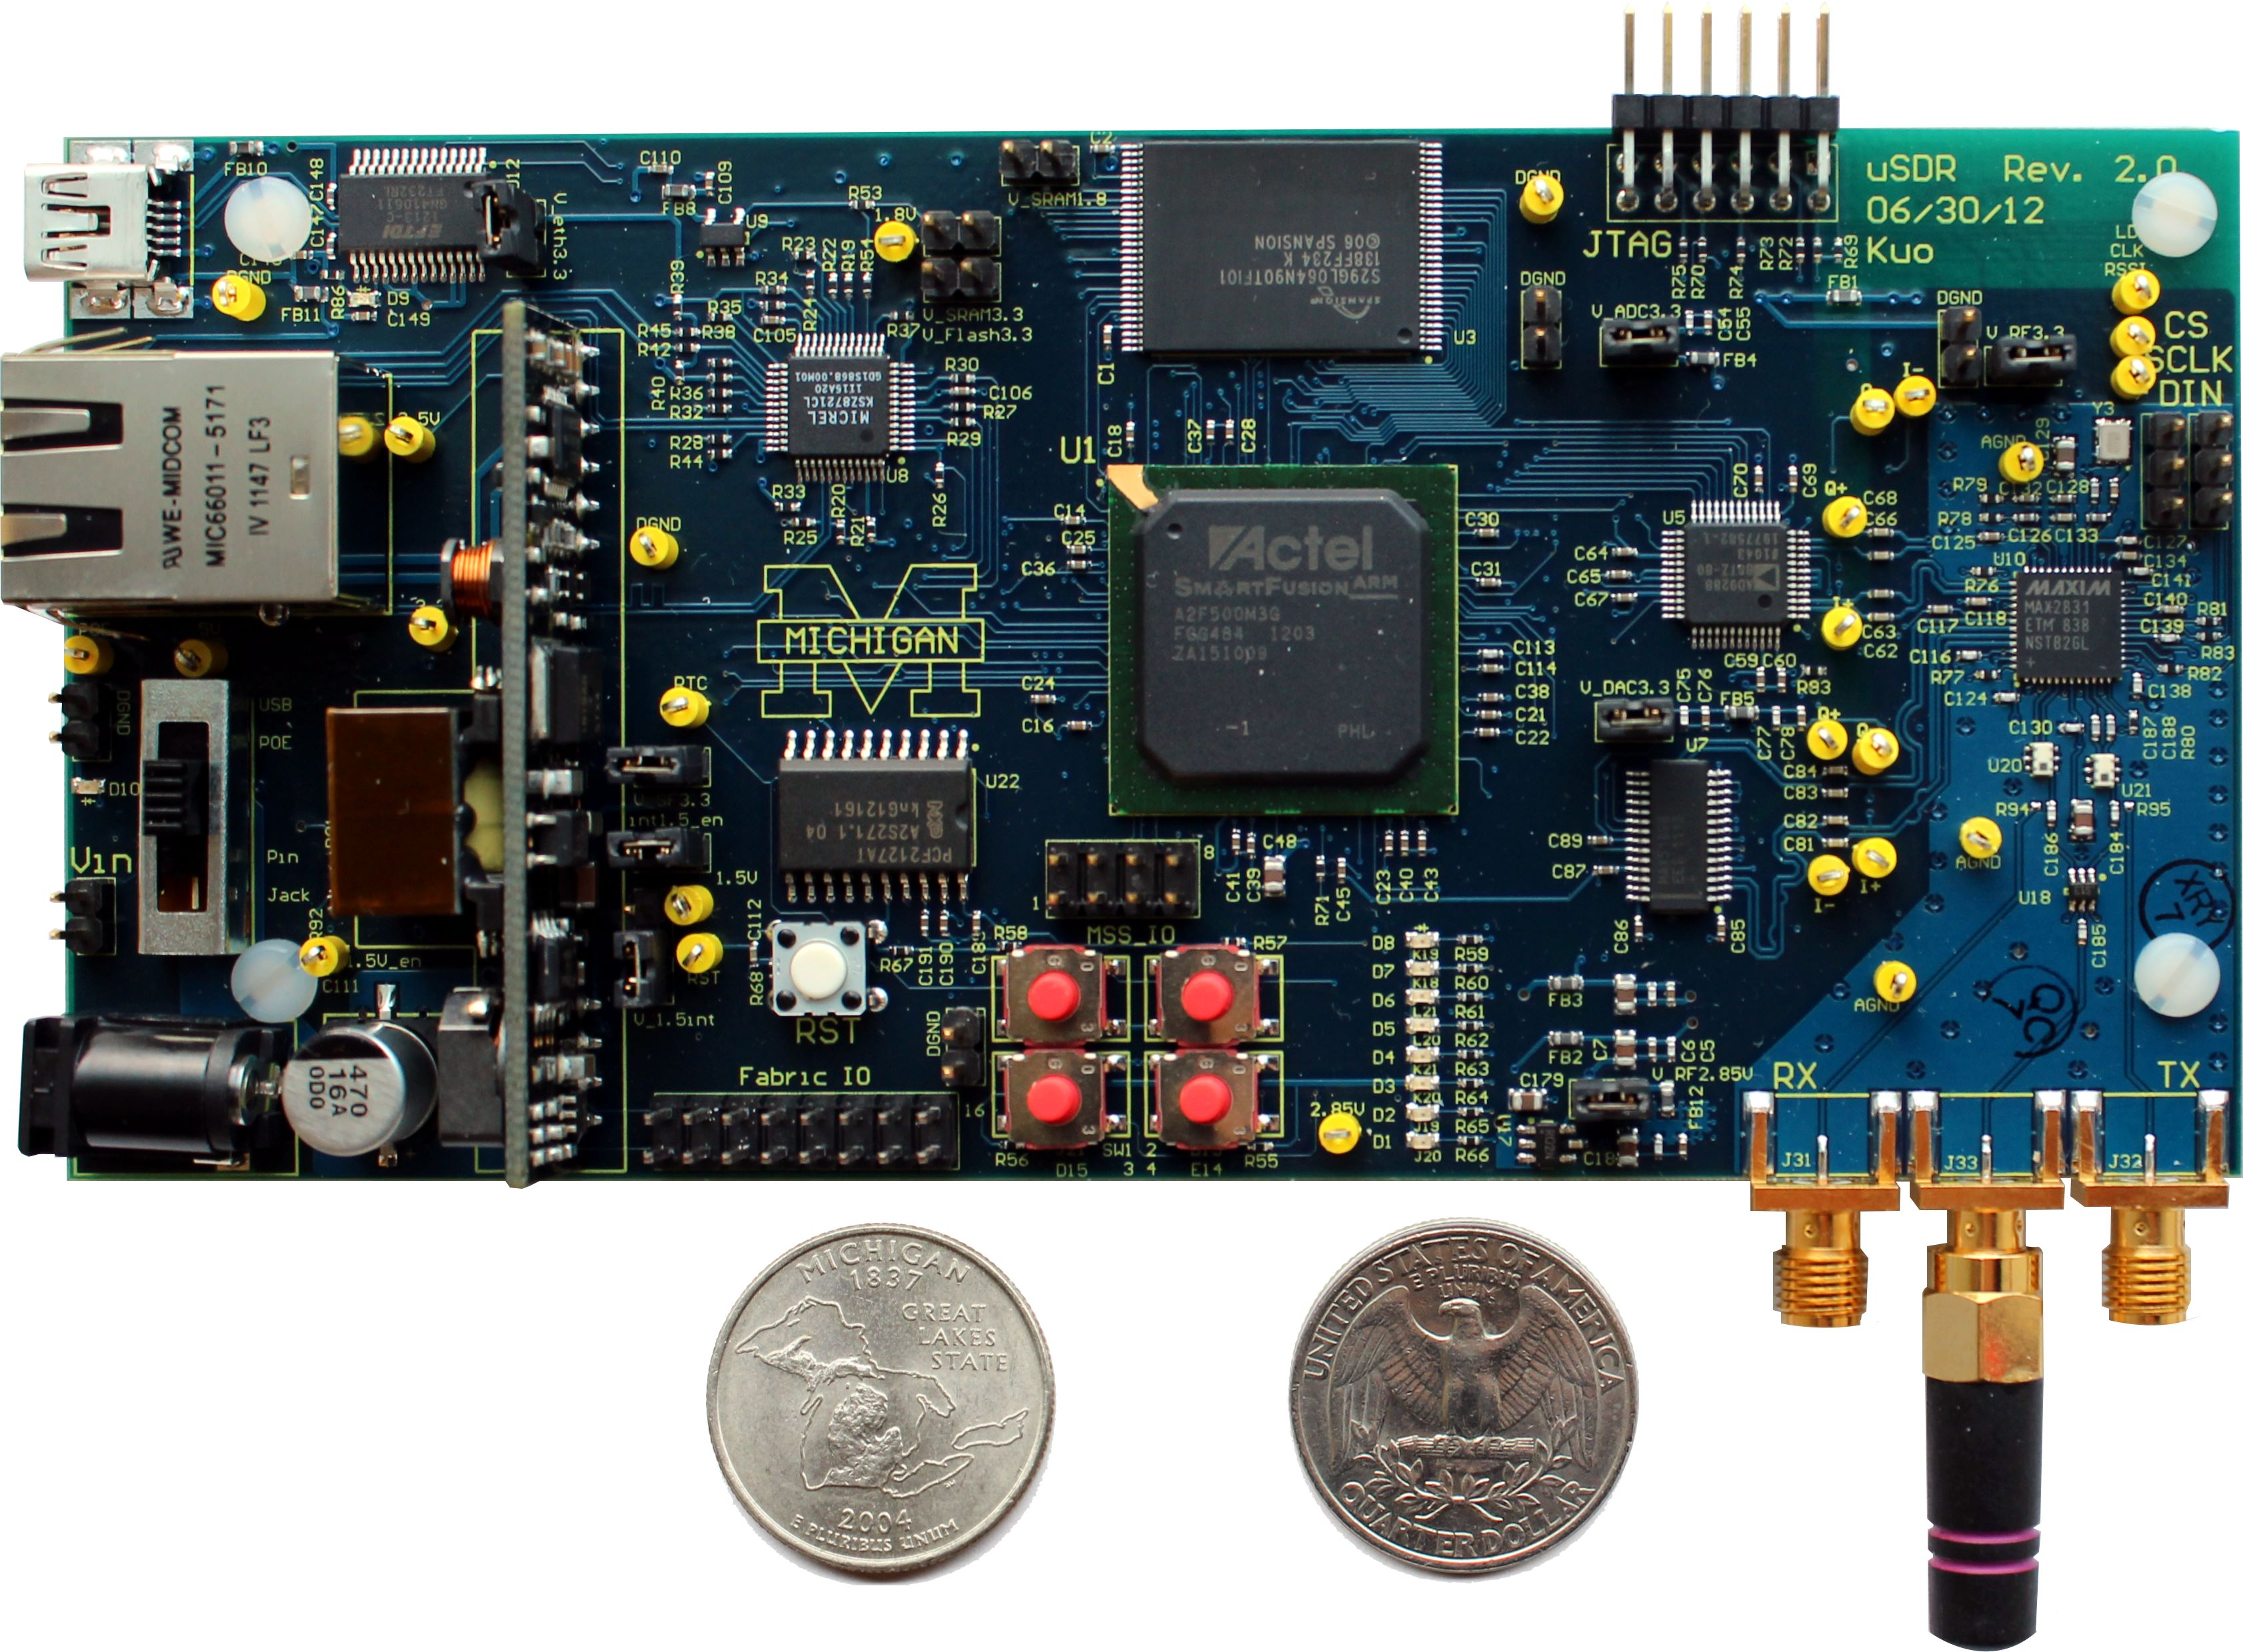
\includegraphics[width=0.6\columnwidth]{sdrv2_scale}
\end{figure}
